\subsection{方法的选择与数据预分析}

考虑到此问题的要求是综合考虑各项指标，得到一个对异常女胎的判断方法，本文决定构建基于机器学习的分类模型。本文选择使用机器学习方法进行求解。数据方面，若孕妇的染色体的非整倍体出现T13、T18、T21中任一异常，那么本文将其标记为“异常女胎”，否则标记为“正常女胎”。同时注意到当妊娠方式为试管婴儿时，仅有 $1$ 个样本出现了染色体非整倍体，样本不足以支撑模型的建立，因此本文不将妊娠方式考虑在因素内。

统计发现，女胎数据染色体的非整倍体分布中，胎儿患 T18 与 T13 的比重相近，T21 的比重较大，约为 T18、T13 的四倍。

\begin{figure} [H]
    \centering
    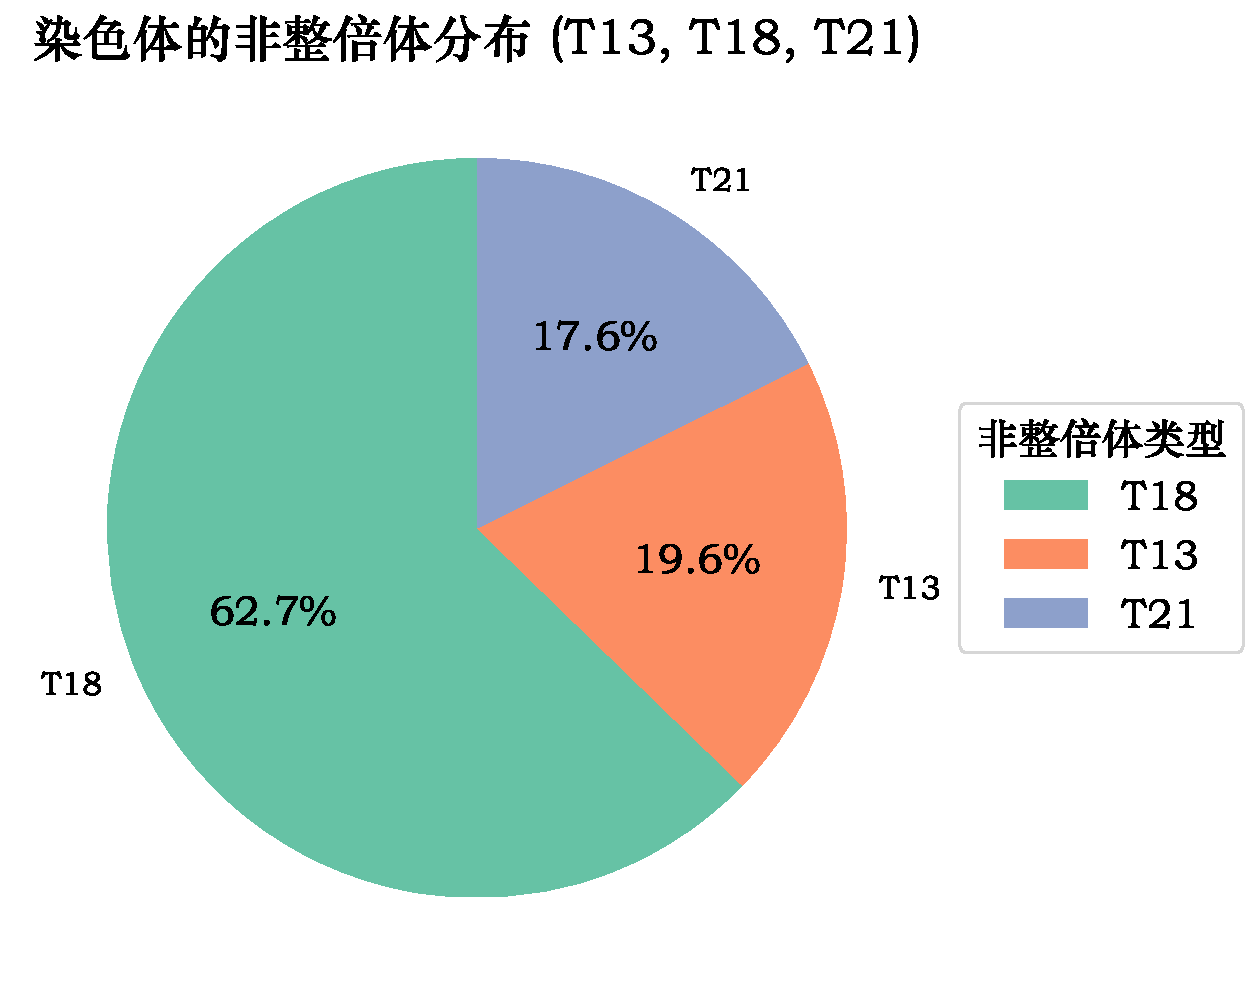
\includegraphics[width=0.4\textwidth]{chapters/Q4/images/非整倍体扇形图.pdf}
    \caption{非整倍体扇形图}
    \label{fig:非整倍体扇形图}
\end{figure}

为了直观地探索各个特征对女胎异常的区分能力，本文采用核密度估计绘制每个特征的平滑概率分布图。通过在同一图表上叠加对比正常样本与异常样本的分布（图 \ref{fig:核心指标对比图}，其余非核心指标见附录图 \ref{fig:其他指标对比图}），发现绝大多数特征的分布曲线都高度重合，而仅在13号、18号、21号及 X 染色体的浓度这几个关键指标上，异常样本的分布曲线显著地向高分区域偏移，可合理猜测X染色体浓度是用于判定女胎异常的最显著特征。

\begin{figure} [H]
    \centering
    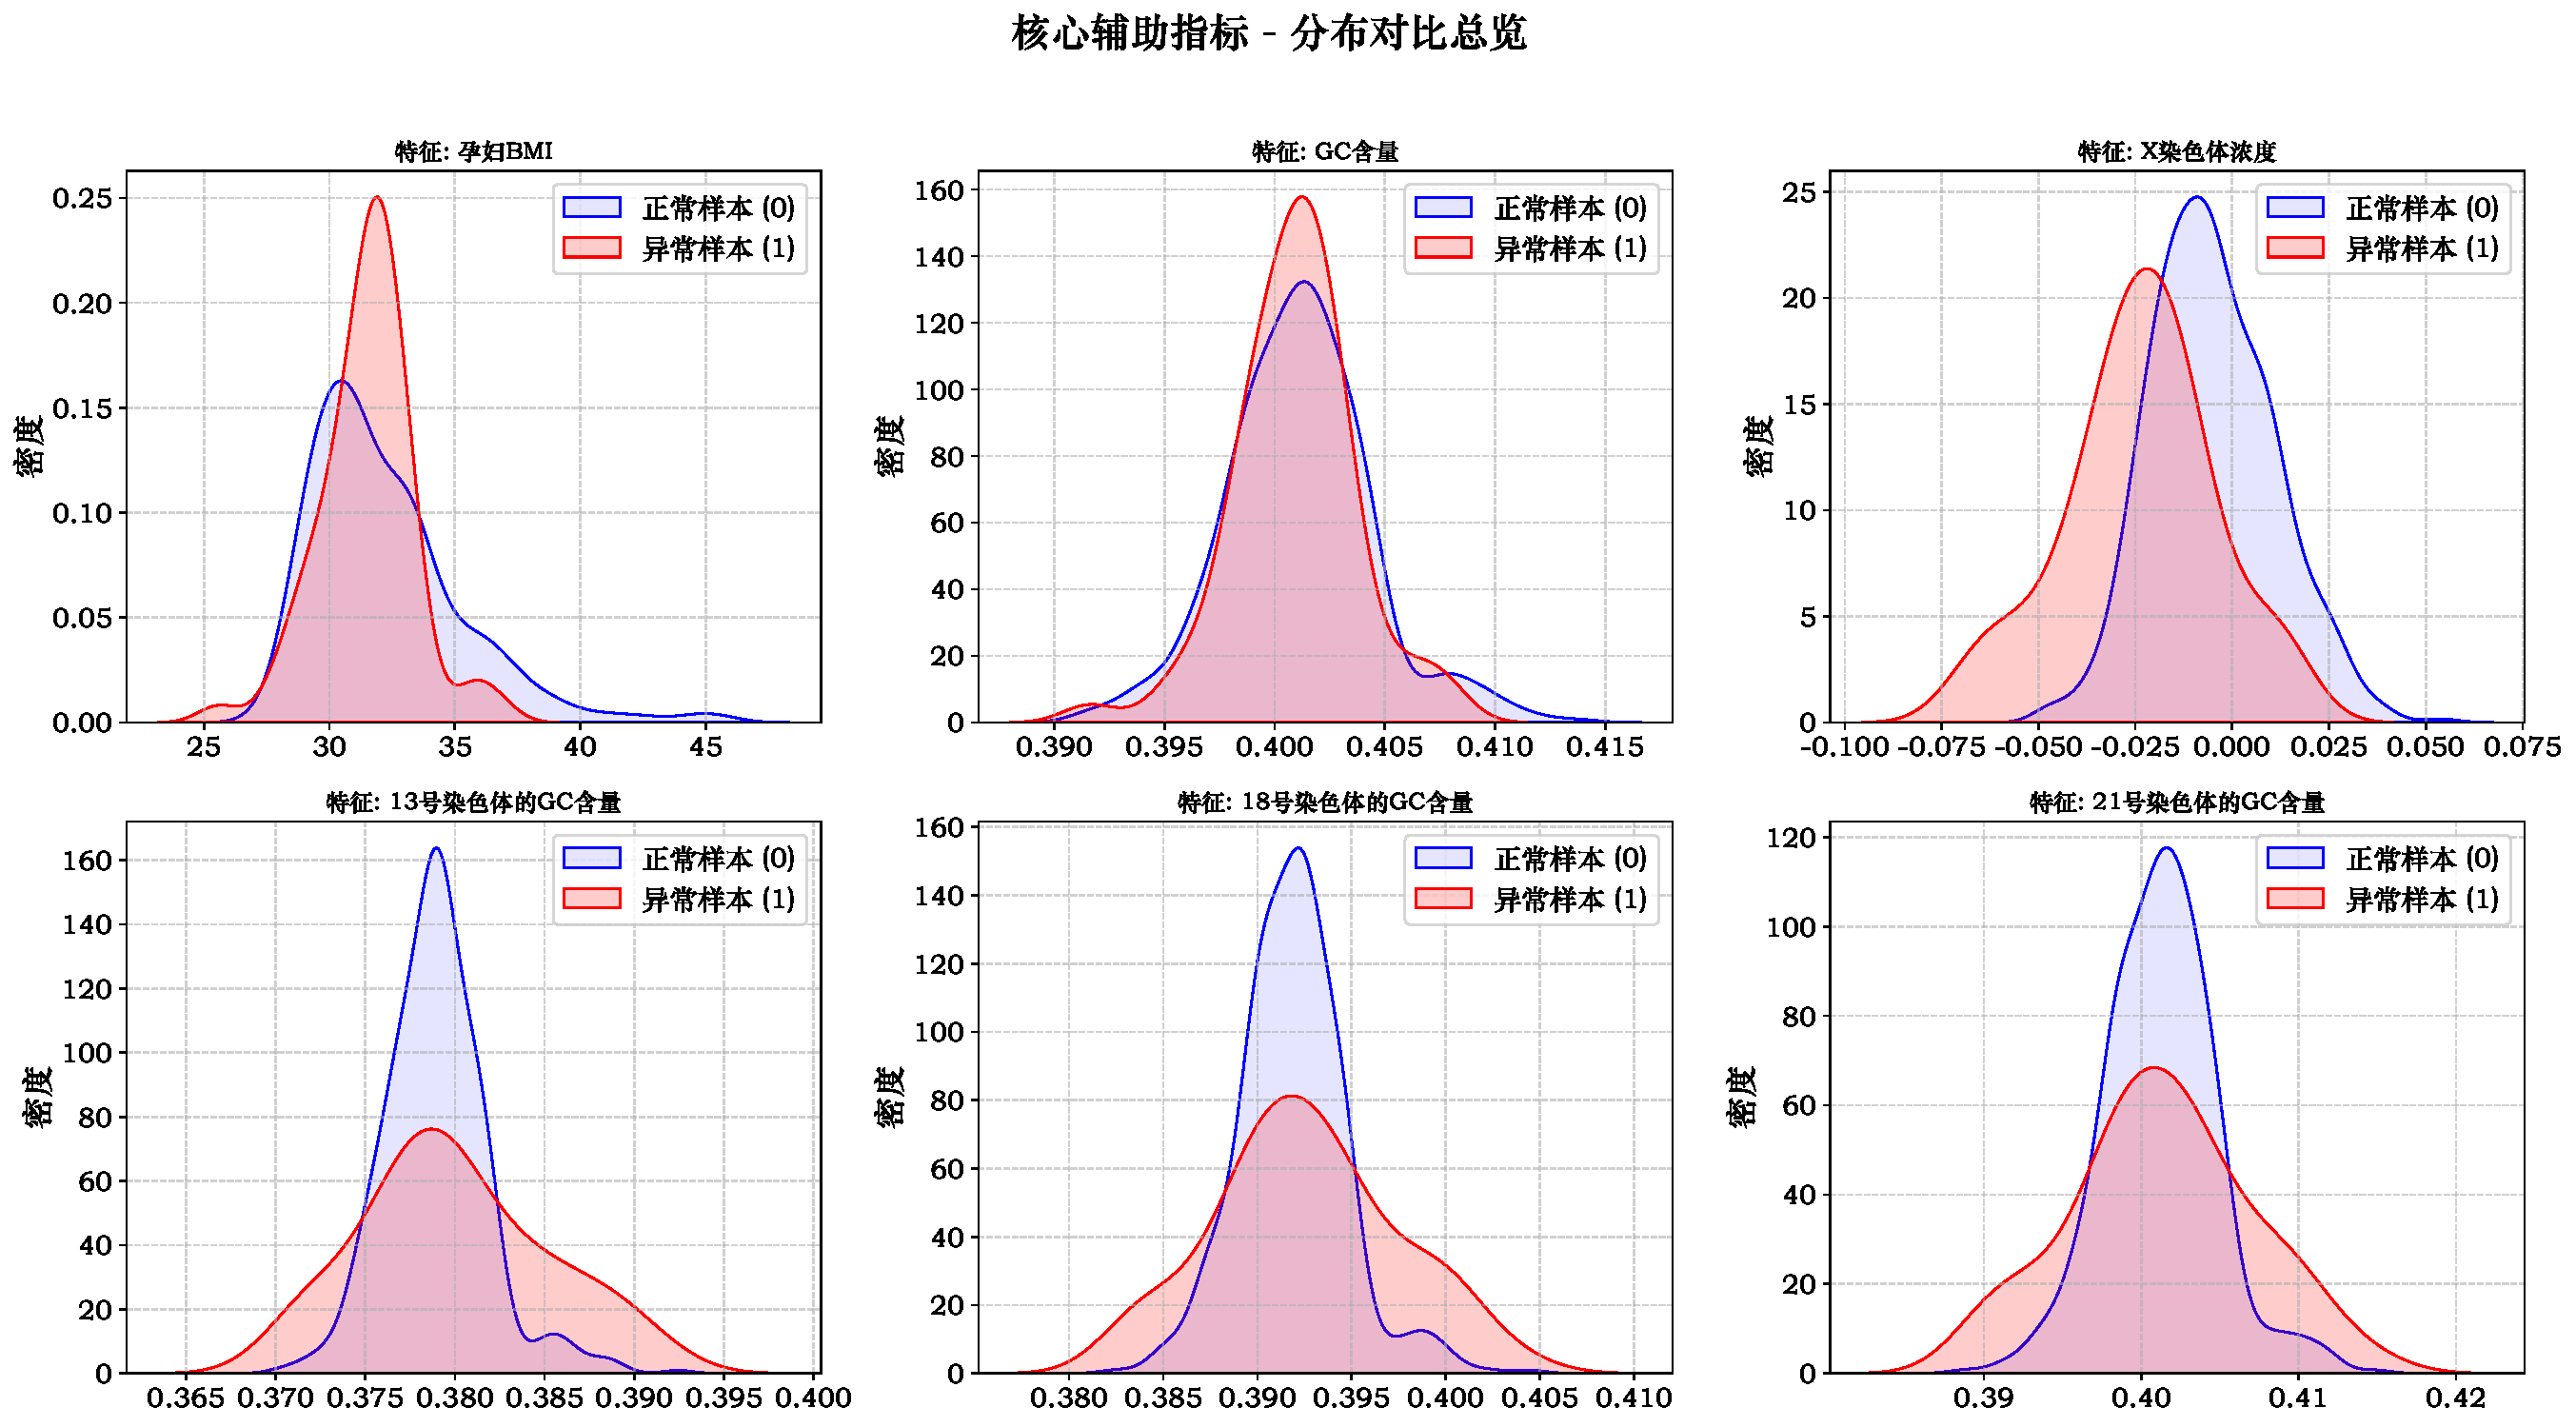
\includegraphics[width=0.9\textwidth]{chapters/Q4/images/核心指标对比图.pdf}
    \caption{核心指标对比图}
    \label{fig:核心指标对比图}
\end{figure}

\subsection{模型优化}

XGBoost是一种高效的梯度提升算法，它的革新主要体现在其对目标函数的重新定义和高效的求解策略上，同时显著提升了训练速度和模型性能。具体来说，XGBoost通过其独特的提升机制，能够捕捉到预测变量之间复杂的、非线性的相互作用关系。在本题中，胎儿是否异常可能并非由单一指标决定，而是多个因素共同作用的结果，而该模型强大的模式识别能力使其能够精确地学习这些复杂的决策边界。在第 $t$ 轮迭代中，XGBoost 需要优化的目标函数由两部分组成，训练损失和正则化项。训练损失和正则化项的定义如下：
\begin{equation}
    \text{Obj}^{(t)} = \sum_{i=1}^{n} l\left(R_i, \hat{y}_i^{(t)}\right) + \sum_{k=1}^{t} \Omega(f_k)  \qquad     \Omega(f_t) = \gamma T + \frac{1}{2}\lambda \sum_{j=1}^{T} w_j^2
\end{equation}
其中，$n$ 是样本总数， $R_i$ 是第 $i$ 个样本“染色体的非整倍体”的真实检测结果，$l(\cdot)$ 是损失函数，用于衡量真实值 $R_i$ 与预测值 $\hat{y}_i^{(t)}$ 之间的差异，$\Omega(f_k)$ 是第 $k$ 棵树的正则化项，$T$ 是树 $f_t$ 的叶子节点数量，$w_j$ 是第 $j$ 个叶子节点的权重（即分数），$\gamma$ 和 $\lambda$ 是控制复杂度的超参数。

注意到附件中异常女胎样本远少于正常样本，直接使用标准XGBoost模型可能会导致对异常胎儿的识别能力不足。当某一类别的样本数量占据绝对优势时，模型会发现将所有样本都预测为多数类，便可以轻易获得非常高的准确率。这种现象导致模型对异常样本的识别能力极差。Zhang et al.在研究中指出，XGBoost算法在直接处理类别不平衡的数据时，其分类效果往往并不理想，可能会对少数类样本产生较高的误分类率\cite{zhang2022research}。因此我们需要对数据进行采样处理，将异常样本和正常样本的数量调整到相近水平。

\subsection{数据采样}

本文最初考虑采用随机上采样、随机下采样方法来使异常女胎的个数与正常女胎的个数相当。随机上采样是随机复制少数类样本，使正负样本数量达到平衡；随机下采样是随机丢弃多数类样本以实现平衡。然而在实际应用中，本文发现随机上采样和随机下采样的效果并不理想。由于异常样本过少，随机上采样会对少数类进行过多的复制，导致模型过拟合，虽然准确率高，但本文发现其对异常样本的识别能力并不强；基于同样的原因，随机下采样可能丢失多数类的重要信息，导致模型的识别能力不足，因此查阅相关文献后，本文决定选用SMOTE\cite{DeepSeek_2}对数据进行处理。

SMOTE的核心思想并非简单地复制少数类实例，而是通过在特定邻域内的几个少数类实例之间进行插值而创建数据点。该算法的计算基于数据的特征值及其关系，而不是将数据点作为一个整体来考虑\cite{fernandez2018smote}。但是SMOTE的短板在于过度泛化，在创建数据的时候可能也会产生噪声数据，因其无法区分不同类别。而Tomeklink是去除多数类中噪声数据的一种方法，可以清除具有相似特征和重叠的多数类中的噪声数据。但作为欠采样方法，Tomeklink移除的样本数量有限，对于严重不平衡的数据集，其改善效果可能不足在实际实现中。Tomeklink和SMOTE过采样结合起来，比单独使用两种方法的效果更好\cite{hairani2023improvement}，因此本文采用这种方法对数据进行采样。

\subsection{模型建立与求解}
本文使用Python的XGBoost库来实现XGBoost分类模型。首先将数据集划分为训练集和测试集，其中，测试集在整个模型训练和优化过程中保持不可见，仅用于最终评估模型的性能。为确保划分后的训练集和测试集中异常样本的比例与原始数据一致，本文采用了\textbf{分层抽样}的方法。随后，将前述的\textbf{SMOTETomek方法}应用于训练集，生成一个类别均衡的、用于模型训练的新数据集。测试集则保持其原本的样本分布，以模拟模型在真实世界数据上的表现，训练流程图如图 \ref{fig:训练流程图} 所示。

\begin{figure}[H]
    \centering
    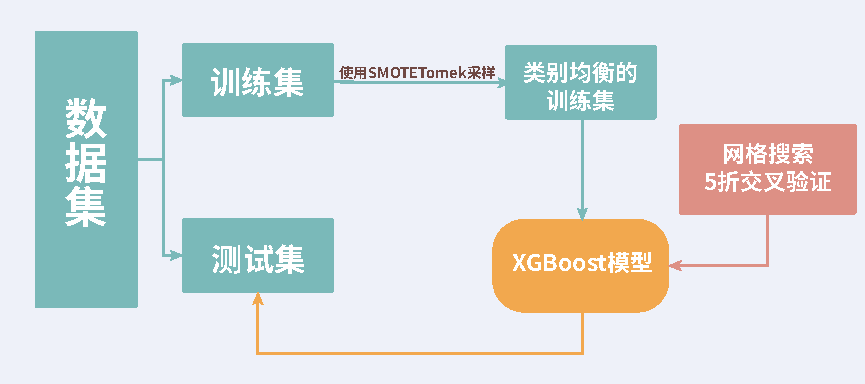
\includegraphics[width=0.5\textwidth]{chapters/Q4/images/xgboost训练流程.pdf}
    \caption{训练流程图}
    \label{fig:训练流程图}
\end{figure}

为了寻找到XGBoost模型的最佳性能，本文将网格搜索与5折交叉验证相结合对模型的关键超参数进行寻优。考虑到在临床诊断中，将异常胎儿误判为正常（即\textbf{漏报，假阴性}）带来的后果是巨大的，而误将正常胎儿误判为异常（即\textbf{误报，假阳性}）的代价相对可控\cite{odibo2005cost}，漏报比误报的代价更大，因此本文选择召回率(Recall)作为网格搜索过程中的核心评估指标。在找到最优超参数组合后，将模型经过在SMOTETomek采样处理后的完整训练集上训练，得到最终的XGBoost分类模型，性能评估报告如图 \ref{tab:performance_report} 所示，数据情况与模型混淆矩阵如图 \ref{fig:数据情况与模型表现情况图} 所示：
\begin{figure}[H]
    \centering
    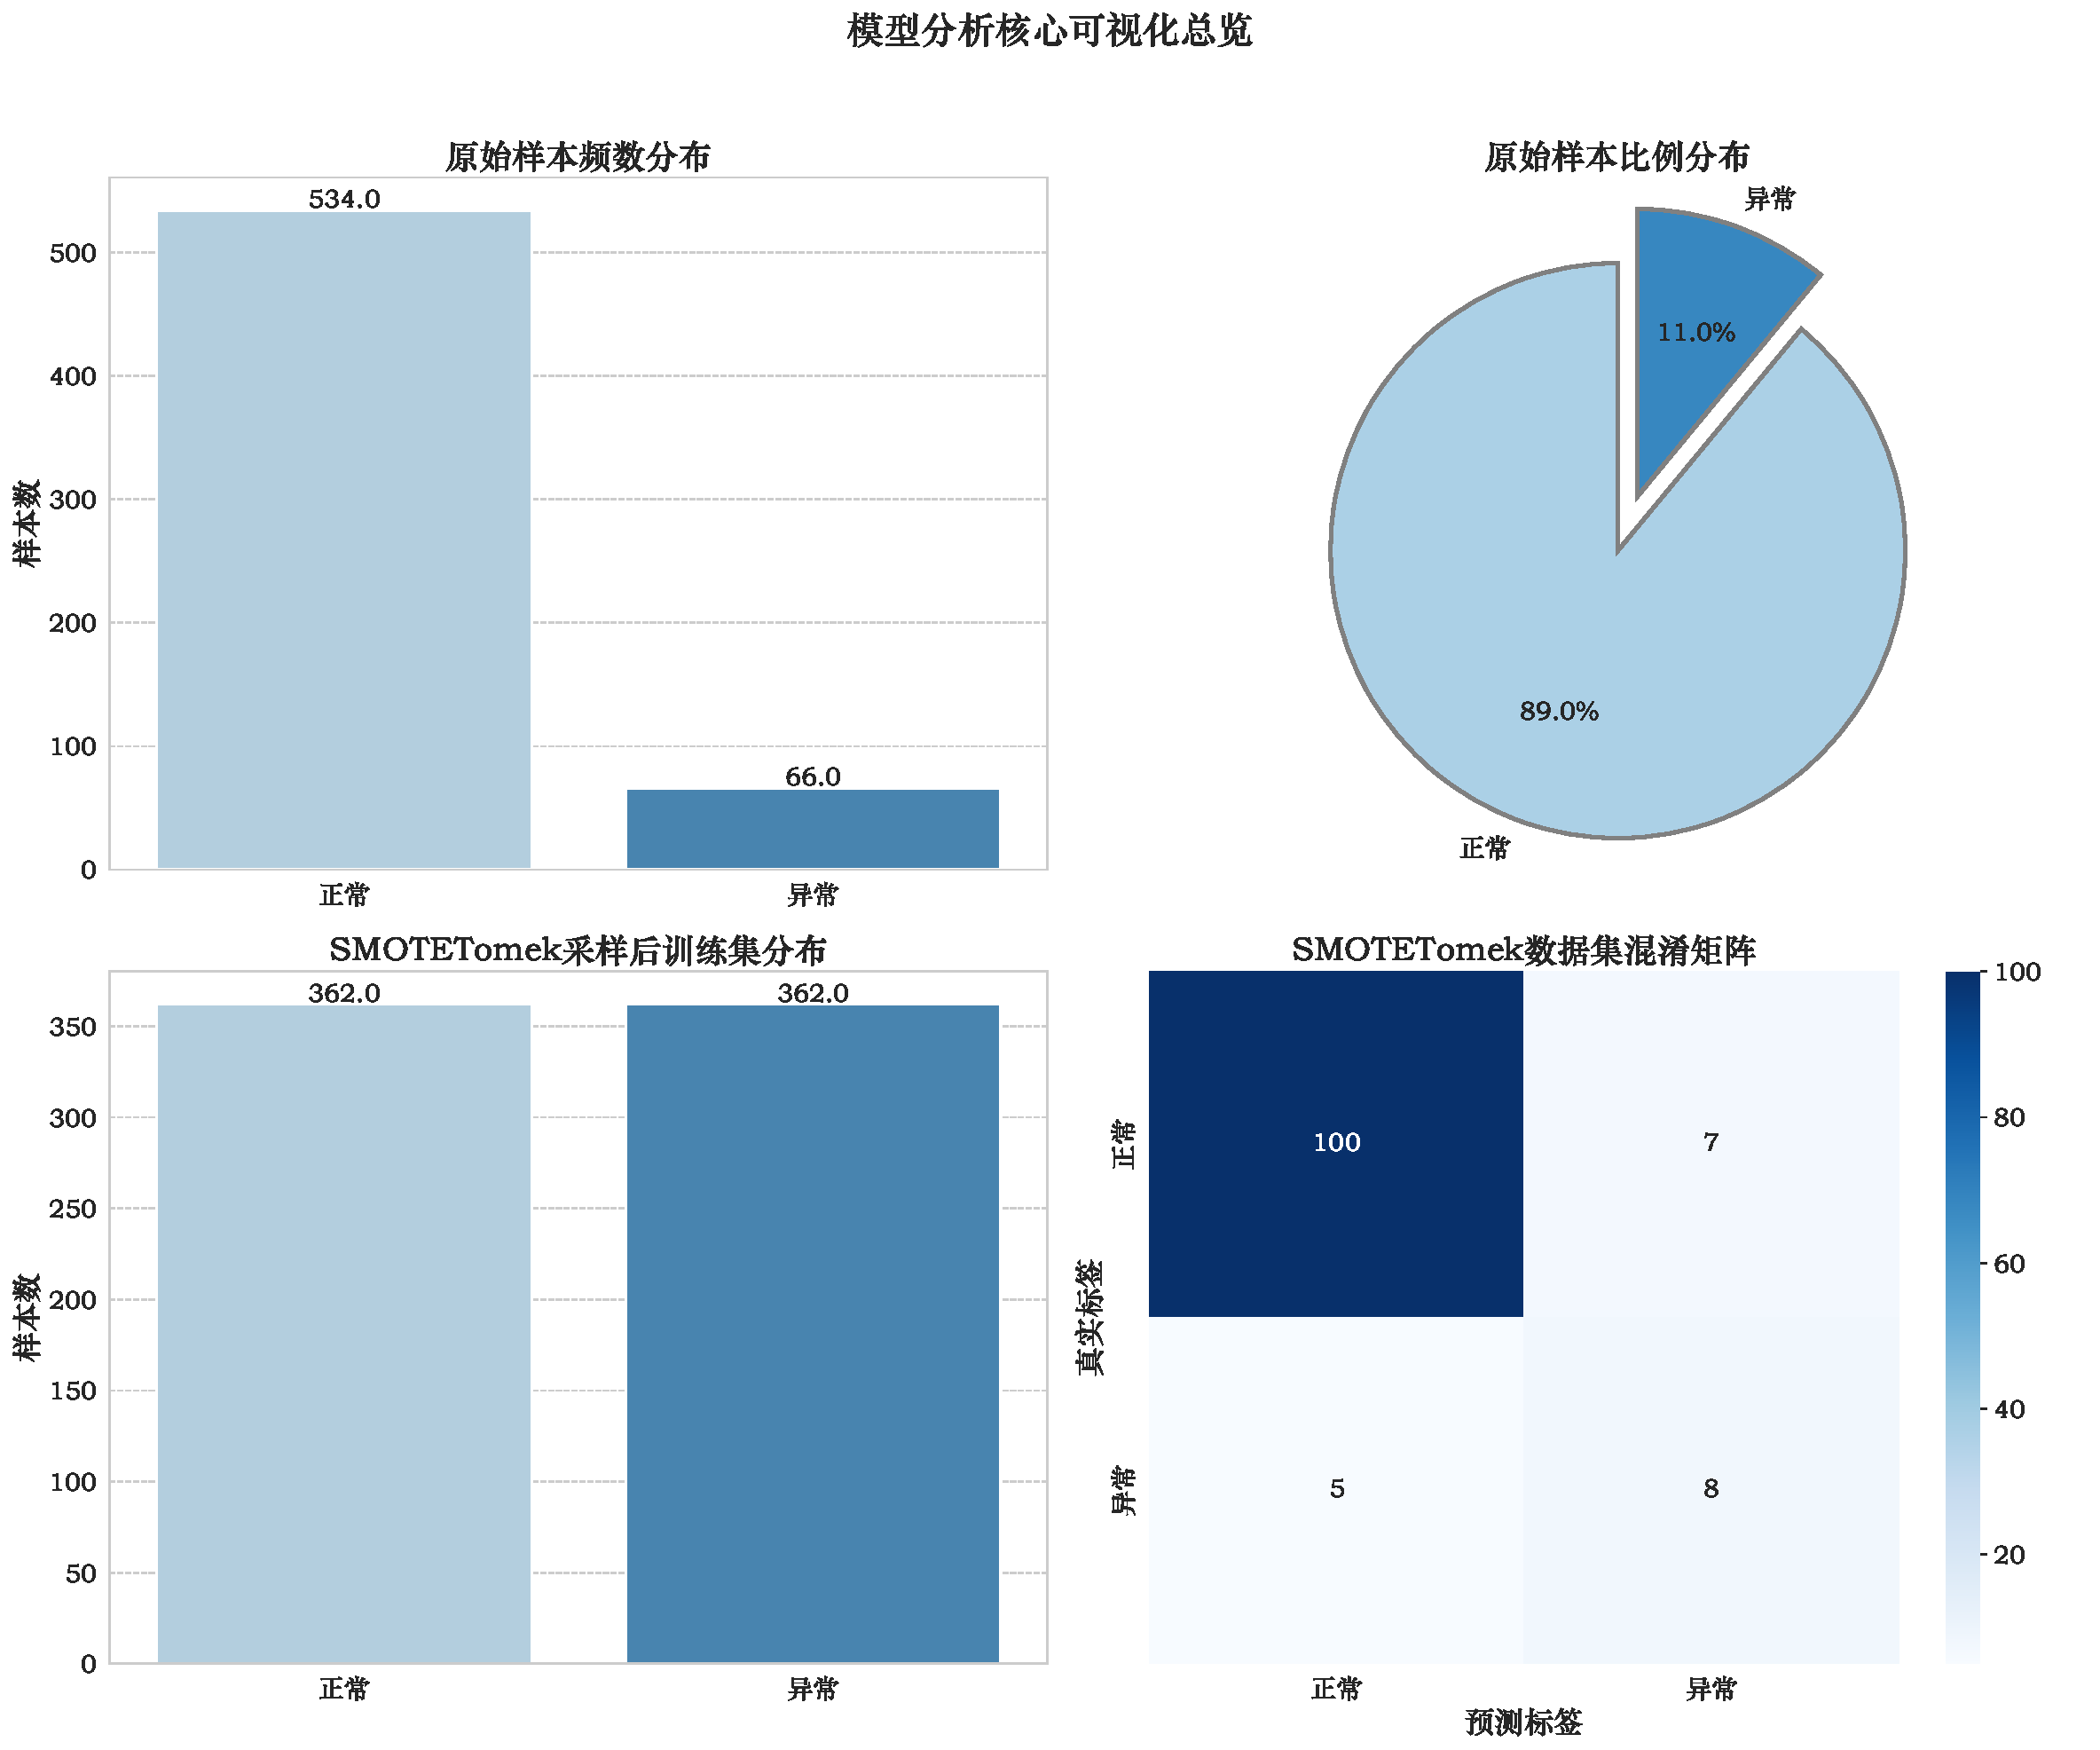
\includegraphics[width=0.65\textwidth]{chapters/Q4/images/核心可视化总览.pdf}
    \caption{数据情况与模型表现情况图}
    \label{fig:数据情况与模型表现情况图}
\end{figure}

\begin{table}[H]
    \centering
    \caption{分类模型性能评估报告}
    \label{tab:performance_report}
    \begin{tabular}{lcccc}
        \toprule
        \textbf{}             & \textbf{Precision} & \textbf{Recall} & \textbf{F1-score} & \textbf{Support} \\
        \midrule
        \textbf{类别 0}         & 0.95               & 0.93            & 0.94              & 107              \\
        \textbf{类别 1}         & 0.53               & 0.62            & 0.57              & 13               \\
        \midrule
        \textbf{accuracy}     &                    &                 & 0.90              & 120              \\
        \textbf{macro avg}    & 0.74               & 0.77            & 0.76              & 120              \\
        \textbf{weighted avg} & 0.91               & 0.90            & 0.90              & 120              \\
        \bottomrule
    \end{tabular}
\end{table}

同时我们也进行了特征的重要性分析，结果如图 \ref{fig:特征重要性} 所示。可以看出，X染色体浓度的特征重要性最高，这与我们前面通过核密度估计所观察到的结果是一致的。

\begin{figure} [H]
    \centering
    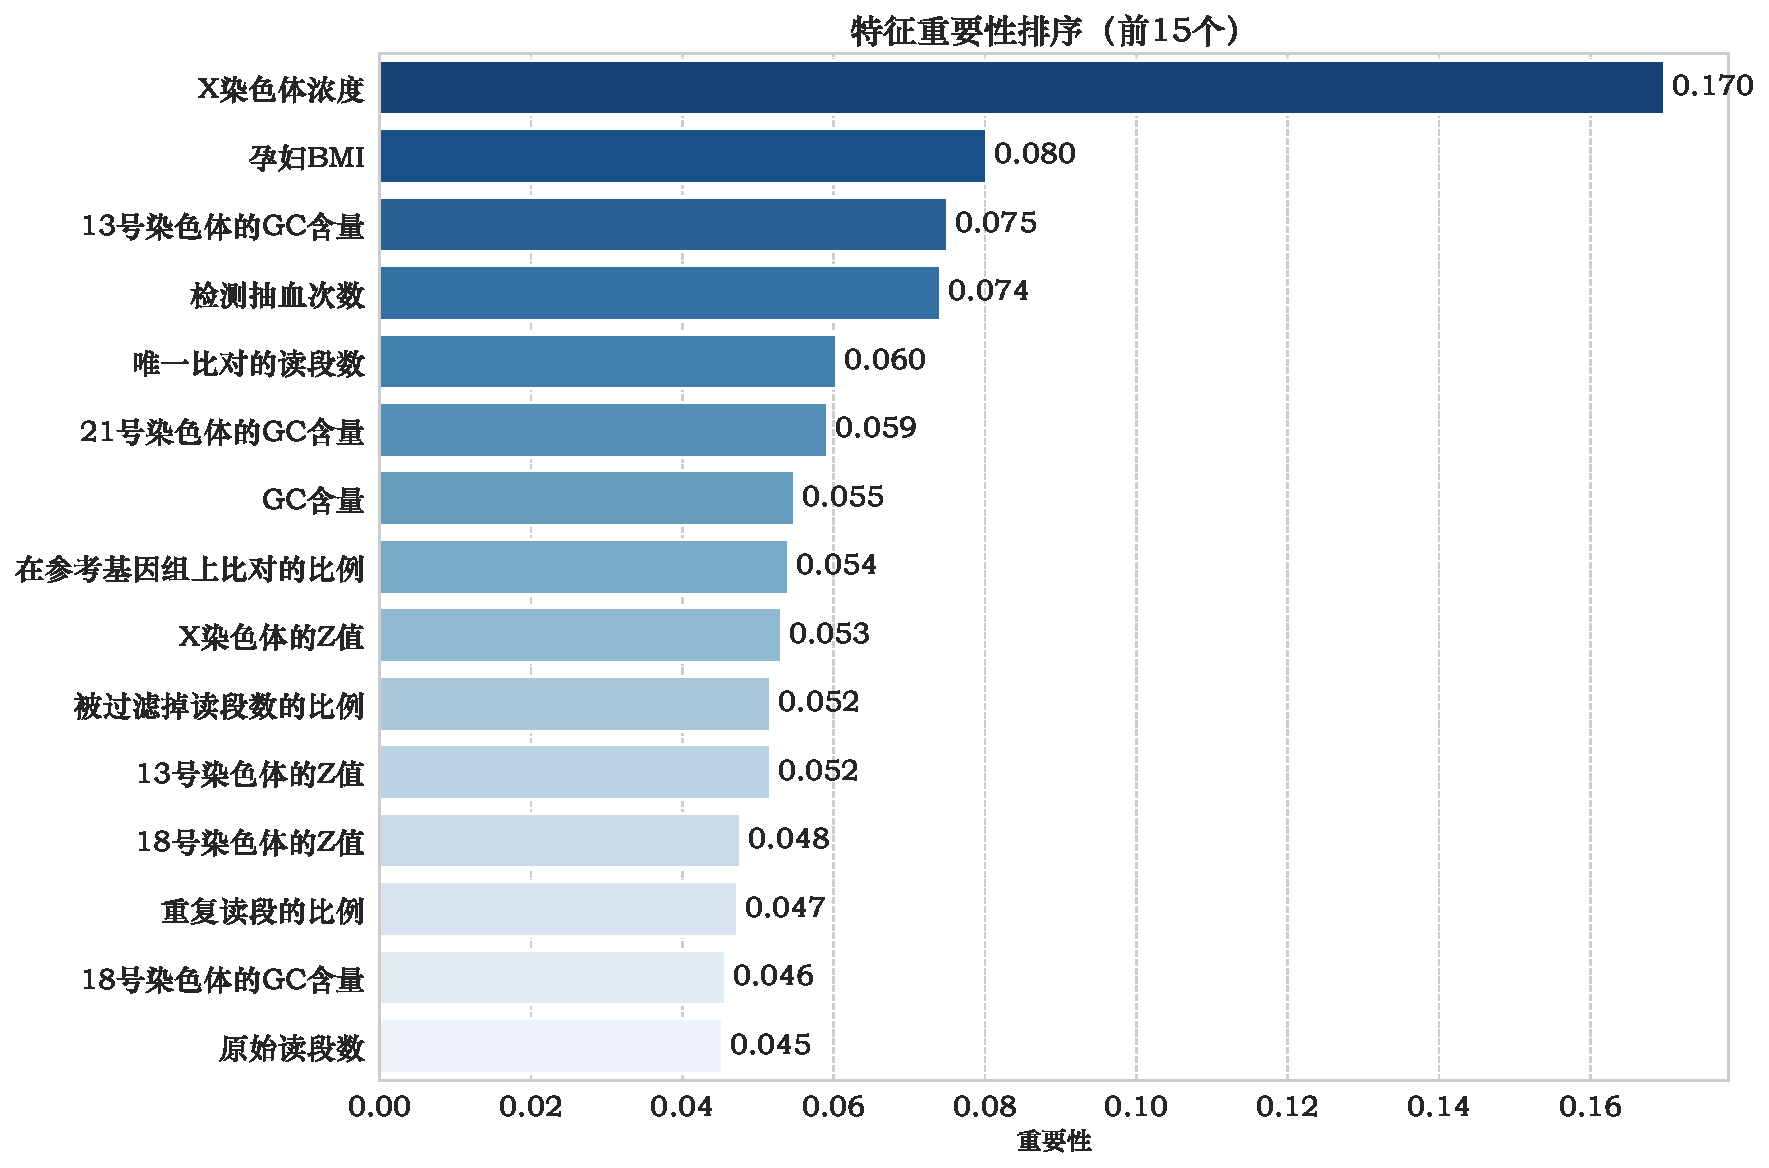
\includegraphics[width=0.7\textwidth]{chapters/Q4/images/特征重要性.pdf}
    \caption{特征重要性}
    \label{fig:特征重要性}
\end{figure}

\subsection{判定预测方法}


本文构建的XGBoost模型在完成预测后，并不会直接输出“异常”或“正常”的二元标签，而是给出一个介于 $[0, 1]$ 之间的连续概率值。该概率值代表了模型预测某个样本为“异常”的可信度。因此，我们需要设定一个\textbf{决策阈值}，当模型输出的概率大于等于该阈值时，则将样本判定为“异常”，反之则为“正常”。因此，选择一个科学、合理的决策阈值，是本判定方法能够应用于实践的关键一步。

为了找到能够最好地平衡“不漏诊”和“不误诊”这对矛盾需求的阈值，本文选择寻找F1值最高值对应的概率值。而要计算F1，也需要\textbf{精确率}和\textbf{召回率}这两个核心评估指标。

\textbf{精确率}是所有被预测为“异常”的样本中，真异常样本的比例，即：
\begin{equation}
    \text{Precision} = \frac{\text{TP}}{\text{TP} + \text{FP}}
    \label{eq:precision}
\end{equation}
其中TP是真正例，FP是假正例。高精确率意味着模型的预测结果误报率低。

\textbf{召回率}是所有真正是“异常”的样本中，被模型成功预测出来的比例。即：
\begin{equation}
    \text{Recall} = \frac{\text{TP}}{\text{TP} + \text{FN}}
    \label{eq:recall}
\end{equation}
其中FN是假反例。高召回率意味着模型的漏报率低。

\textbf{F1分数}是精确率和召回率的调和平均数，是同时考虑这两个指标的综合性评价指标。其计算公式为：
\begin{equation}
    F_1 = 2 \cdot \frac{\text{Precision} \cdot \text{Recall}}{\text{Precision} + \text{Recall}}
    \label{eq:f1_score}
\end{equation}

只有当精确率和召回率二者都较高时，F1分数才会高，因此选择F1分数最高值即能得到在“误判”和“漏判”两方面兼顾的最佳阈值。

本文的最优阈值判定方法为遍历所有可能的决策阈值，计算出在每一个阈值下模型在测试集上的精确率和召回率，并由此得到对应的F1分数。最终选取能够使\textbf{F1分数达到最大值}的那个阈值作为最终的判定标准，计算过程如图 \ref{fig:阈值选择} 所示。经过计算，本文得到的最优决策阈值为 $0.8128$，对应的最高F1分数是$0.571$。

\begin{figure}[H]
    \centering
    
\includegraphics[width=0.8\textwidth]{chapters/Q4/images/阈值选择可视化.pdf}
    \caption{阈值选择}
    \label{fig:阈值选择}
\end{figure}

为了能够通过给定单条数据判定女胎是否异常，本文能够提供基于训练好的分类模型的预测交互。在模型训练代码中，训练结束后可允许用户输入 $16$ 个关键特征参数，模型将基于这些输入数据计算并输出胎儿异常的风险概率。模型输出两个概率值：正常概率和异常概率，异常概率即为胎儿存在染色体非整倍体异常的风险评估值，该数值介于 $0 \sim 1$ 之间，若异常概率大于上文所计算出的最优决策阈值 $0.8128$，则判定为“异常”，否则判定为“正常”。